\subsection{Segment Registers}
\label{sec:segments}

The price of the Intel 64-bit architecture's widespread adoption was the
ability to run software targeting the older 32-bit architecture side-by-side
with 64-bit software \cite{cnet2005itanium}, which resulted in some warts in
the 64-bit architecture. While most warts are not material to the understanding
and operation of SGX, the 64-bit architecture's segment registers and vestigial
segmentation model must be understood. Therefore, this section covers the
segmentation concepts needed to understand SGX.

The semantics of the Intel architecture's instructions include the implicit use
of a few segments which are loaded into the processor's
\textit{segment registers} shown in Figure~\ref{fig:cpu_registers}. Code
fetches use the \textit{code segment} (CS).  Instructions that reference the
stack implicitly use the \textit{stack segment} (SS). Memory references
implicitly use the \textit{data segment} (DS) or the \textit{destination
segment} (ES). Via segment override prefixes, instructions can be modified to
use the unnamed segments FS and GS for memory references.

Modern operating systems effectively disable segmentation by covering the
entire addressable space with one segment, which is loaded in CS, and one data
segment, which is loaded in SS, DS and ES. The FS and GS registers store
segments covering \textit{thread-local storage} (TLS).

% Segment Selectors: SDM S 3.4.2
% Segment Registers: SDM S 3.4.3

Due to the Intel architecture's 16-bit origins, segment registers are exposed
as 16-bit values, called \textit{segment selectors}. The top 13 bits in a
selector are an index in a \textit{descriptor table}, and the bottom 2 bits are
the selector's ring number, which is also called requested privilege level
(RPL) in the Intel documentation. Also, modern system software only uses rings
0 and 3 (see \S~\ref{sec:rings}).

% Segment Loading Instructions in IA-32e Mode: SDM S 3.4.4
% Limit Checking in 64-bit Mode: SDM S 5.3.1
% Privilege Levels: SDM S 5.5

Each segment register has a hidden \textit{segment descriptor}, which consists
of a \textit{base address}, \textit{limit}, and type information, such as
whether the descriptor should be used for executable code or data.
Figure~\ref{fig:cpu_segment} shows the effect of loading a 16-bit selector into
a segment register. The selector's index is used to read a descriptor from the
descriptor table and copy it into the segment register's hidden descriptor.

\begin{figure}[hbt]
  \centering
  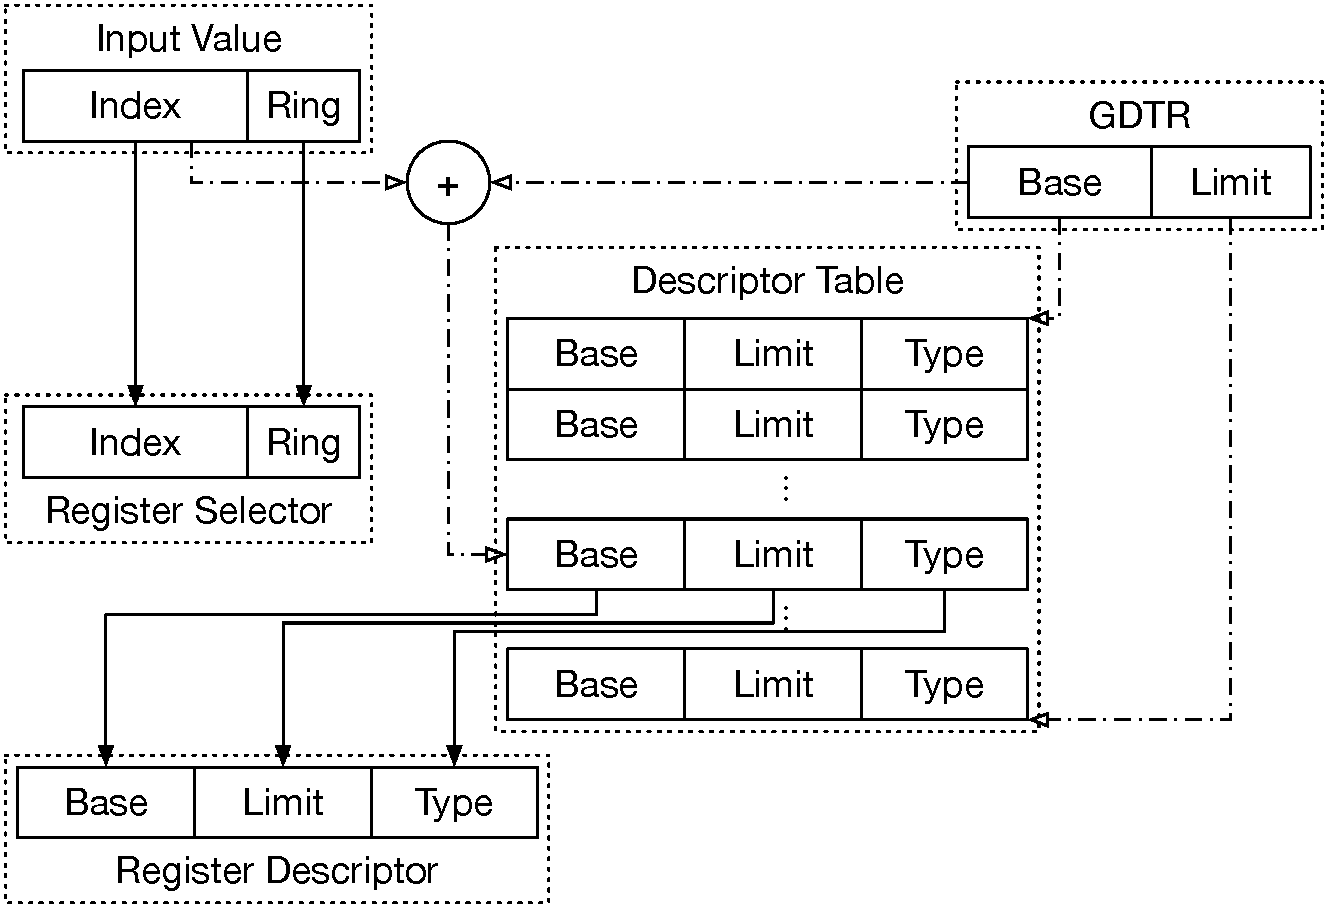
\includegraphics[width=85mm]{figures/cpu_segment.pdf}
  \caption{
    Loading a segment register. The 16-bit value loaded by software is a
    selector consisting of an index and a ring number. The index selects a GDT
    entry, which is loaded into the descriptor part of the segment register.
  }
  \label{fig:cpu_segment}
\end{figure}

In 64-bit mode, all segment limits are ignored. The base addresses in most
segment registers (CS, DS, ES, SS) are ignored. The base addresses in FS and GS
are used, in order to support thread-local storage.
Figure~\ref{fig:cpu_segmentation} outlines the address computation in this
case. The instruction's address, named \textit{logical address} in the Intel
documentation, is added to the base address in the segment register's
descriptor, yielding the virtual address, also named \textit{linear address}.
The virtual address is then translated (\S~\ref{sec:paging}) to a physical
address.

\begin{figure}[hbt]
  \centering
  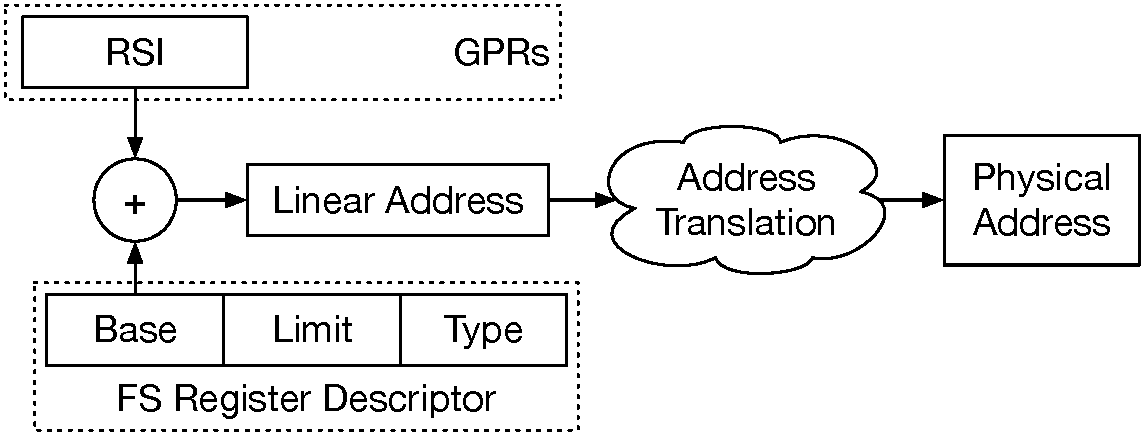
\includegraphics[width=80mm]{figures/cpu_segmentation.pdf}
  \caption{
    Example address computation process for \texttt{MOV FS:[RDX], 0}.  The
    segment's base address is added to the address in RDX before address
    translation (\S~\ref{sec:paging}) takes place.
  }
  \label{fig:cpu_segmentation}
\end{figure}

Outside the special case of using FS or GS to reference thread-local storage,
the logical and virtual (linear) addresses match, so most of this paper uses
the term ``virtual address'' and ignores segmentation.

Even though CS is not used for segmentation, 64-bit system software needs to
load a valid selector into it. The CPU uses the ring number in the CS selector
to track the current privilege level, and uses one of the type bits to know
whether it's running 64-bit code, or 32-bit code in compatibility mode.

% Null Segment Selector Checking: SDM S 5.4.1, S 5.4.1.1

The DS and ES segment registers are completely ignored, and can have null
selectors loaded in them. The CPU loads a null selector in SS when switching
privilege levels, discussed in \S~\ref{sec:faults}.

% Segment Loading Instructions in IA-32e Mode: SDM S 3.4.4
% Segmentation in IA-32e Mode: SDM S 3.2.4

Modern kernels only use one descriptor table, the \textit{Global Descriptor
Table} (GDT), whose virtual address is stored in the GDTR register. Table~
\ref{fig:gdt_layout} shows a typical GDT layout that can be used by 64-bit
kernels to run both 32-bit and 64-bit applications.

\begin{table}[hbt]
  \centering
  \begin{tabular}{| l | l |}
  \hline
  \textbf{Descriptor} & \textbf{Selector}\\
  \hline
  Null (must be unused) & 0 \\
  \hline
  Kernel code & 0x08 (index 1, ring 0) \\
  \hline
  Kernel data & 0x10 (index 2, ring 0) \\
  \hline
  User code & 0x1B (index 3, ring 3) \\
  \hline
  User data & 0x1F (index 4, ring 3) \\
  \hline
  TSS & 0x20 (index 5, ring 0) \\
  \hline
  \end{tabular}
  \caption{
    A typical GDT layout in the 64-bit Intel Architecture.
  }
  \label{fig:gdt_layout}
\end{table}

% TSS Descriptor: SDM S 7.2.2
% TSS Descriptor in 64-bit mode: SDM S 7.2.3
% Task Register: SDM S 7.2.4
% Task Management in 64-bit Mode: SDM S 7.7

The last entry in Table~\ref{fig:gdt_layout} is a descriptor for the
\textit{Task State Segment} (TSS), which was designed to implement hardware
context switching, named \textit{task switching} in the Intel documentation.
The descriptor is stored in the \textit{Task Register} (TR), which behaves like
the other segment registers described above.

Task switching was removed from the 64-bit architecture, but the TR segment
register was preserved, and it points to a repurposed TSS data structure. The
64-bit TSS contains an \textit{I/O map}, which indicates what parts of the I/O
address space can be accessed directly from ring 3, and the
\textit{Interrupt Stack Table} (IST), which is used for privilege level
switching (\S~\ref{sec:faults}).

Modern operating systems do not allow application software any direct access to
the I/O address space, so the kernel sets up a single TSS that is loaded into
TR during early initialization, and used to represent all applications running
under the OS.
